\documentclass[tikz]{standalone}
% https://tex.stackexchange.com/questions/58702/creating-gears-in-tikz

\begin{document}
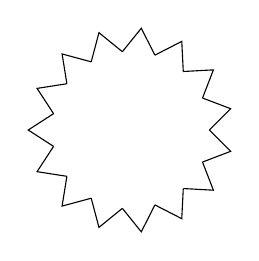
\begin{tikzpicture}
    \def\teeth{15}
    \def\innerRadius{1cm}
    \def\outerRadius{1.3cm}
    \pgfmathsetmacro\angle{360/(2*\teeth)}

    \foreach \i in {1,2,...,\teeth} {
        \draw ({\i*\angle*2}:\innerRadius)
            -- ({(2*\i+1)*\angle}:\outerRadius)
            -- ({(2*\i+2)*\angle}:\innerRadius);
    }
    
\end{tikzpicture}
\end{document}